\subsubsection{分析与准备：分块观测与受限干扰项}

问题二要在同一块晶圆的两条光谱中找出共同的厚度信息，同时把入射角造成的外观差异留在各自模型里。为避免相邻波数点被误当成独立测试，先把主拟合窗口的原始坐标组织成连续区段，再分别安排估计、校准与计分。在$1200$--$3800\ \mathrm{cm}^{-1}$主拟合窗口内，先按波数升序排列观测，再将首末观测之间的序号范围均分为$479$份，分点序号向下取整，连同两端共取$480$个原始坐标点；保留附件给出的波数值，不插值为等距波数网格。
% src:求解/问题2/结果/数据审查.json:主窗口_cm^-1;抽样点数_每角度;抽样索引

这些坐标按顺序每$40$点组成一块，形成$12$个连续块，块号随波数递增。连续块数和训练边界的$20\ \mathrm{cm}^{-1}$保护带均由两角共同使用并预先固定，保护带隔开邻近观测以减轻信息串入。
% src:求解/问题2/结果/数据审查.json:抽样索引
% src:求解/问题2/结果/基准交接.json:训练保护带_cm^-1;折分

训练段估计参数并确定归一化尺度，校准段只校准预测区间半宽，测试段只计分。正式比较采用两折，即两套训练、校准和测试的区段分工，具体块号见表\ref{tab:05}；上一节的五折是在同一组连续块上另行轮换测试区段，用于检查厚度随留段位置的变化，并非另分五个块。图\ref{fig:split}展示两角采用相同波数分组的两折训练、校准和测试安排；这种安排使模型选择、区间校准与预测评价各有来源，不把随机拆行或统一平滑当作独立验证。
% src:求解/问题2/结果/基准交接.json:折分;五折连续留段
% src:交接/图注素材_2.json:1.论文引用建议

\begin{figure}[H]
  \centering
  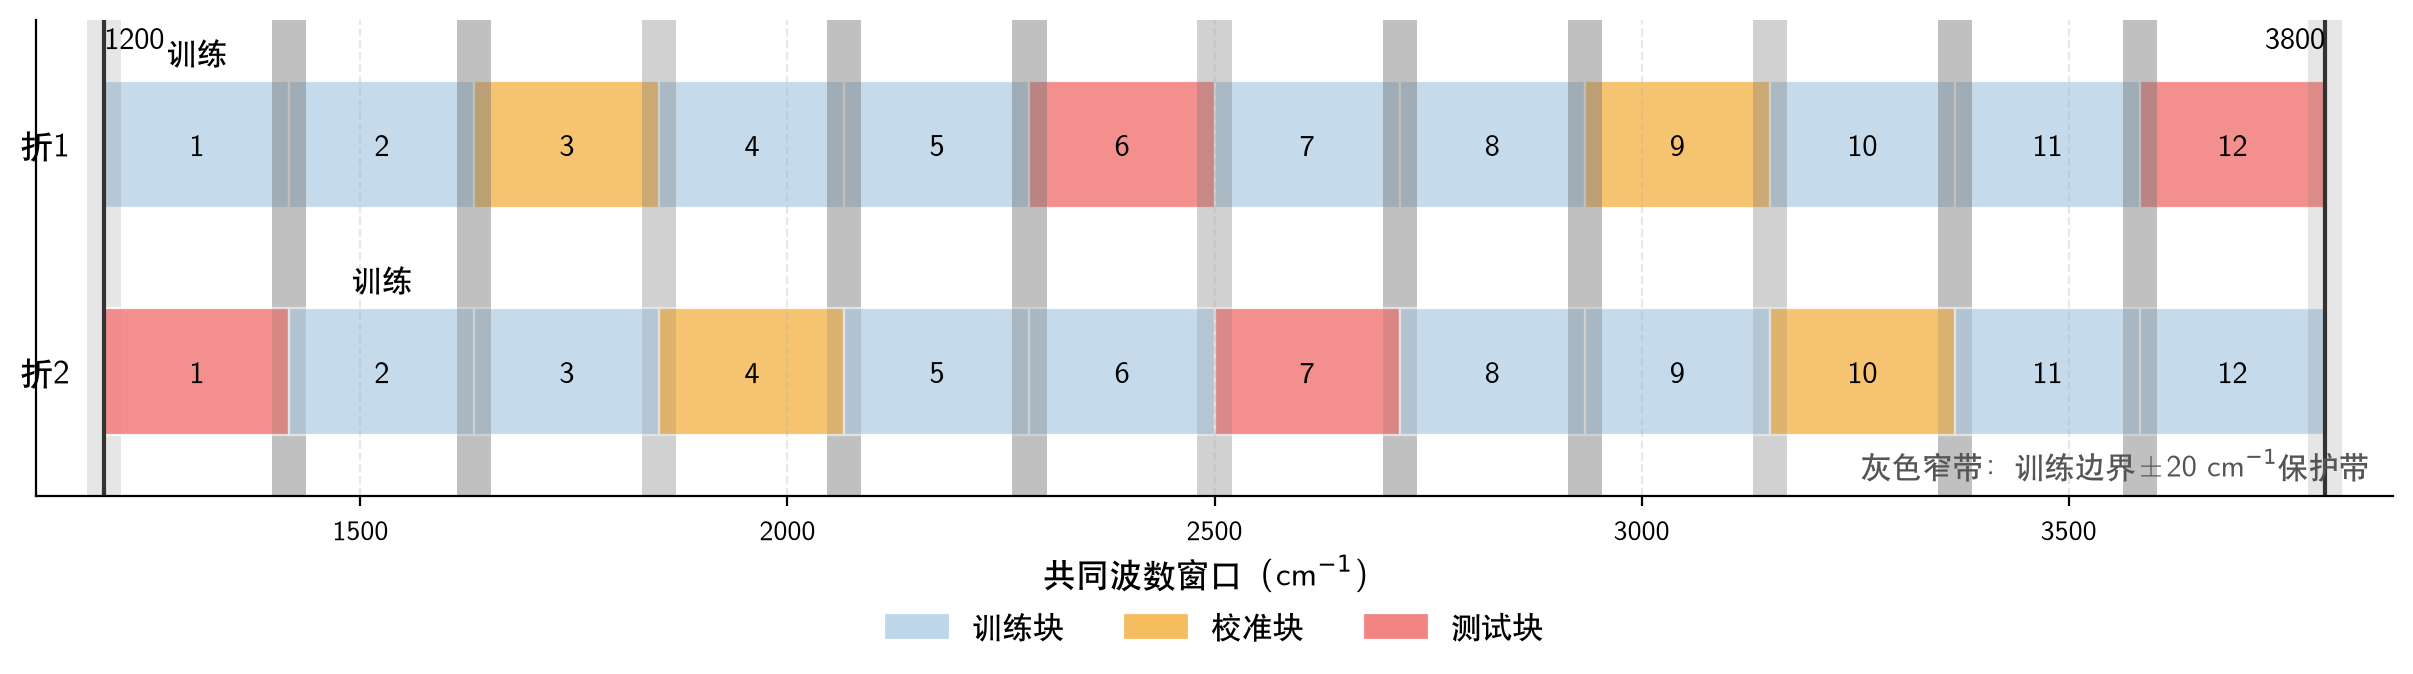
\includegraphics[width=0.8\textwidth,height=35.7mm,keepaspectratio]{../求解/问题2/图片/连续留段隔离拟合与检验.png}
  \caption{两角同步留段的训练校准测试区段}
  \label{fig:split}
\end{figure}

末端$3800$--$4000.122\ \mathrm{cm}^{-1}$另作外层检验，保护窗口为$3750$--$3800\ \mathrm{cm}^{-1}$。
% src:求解/问题2/结果/基准交接.json:末端新留段.0.测试窗口_cm^-1;末端新留段.0.保护窗口_cm^-1

两谱的原始相关系数为$0.9987$，但反射率均方根差仍有$2.14$个百分点。初次以双角高相关评价厚度可靠性，核对后改为同波数双角分组，以训练尺度归一化的留段预测误差比较方法。波数逐行对齐决定双角同步分组，同片物理条件决定共享厚度；原谱高相关包含慢变基线，留段预测用于检验模型对谱形的解释。
% src:交接/数据档案.json:跨文件关系.两两全量核验.0.原始反射率皮尔逊相关系数;跨文件关系.两两全量核验.0.均方根差;跨文件关系.同片分组
% src:交接/实验记录.json:50.尝试;50.现象;50.决定

超界观测来自附件2，共有$262$个反射率超过$100\%$的原值，所在区间与主拟合窗口不相交，点数及波数范围列入表\ref{tab:05}。这些观测不参与主拟合窗口拟合，原文件保持不变。
% src:交接/数据档案.json:文件档案.1.工作表.0.反射率检查.超过百分之百点数;文件档案.1.工作表.0.反射率检查.超过百分之百区段.0.起始波数;文件档案.1.工作表.0.反射率检查.超过百分之百区段.0.终止波数
% src:求解/问题2/结果/数据审查.json:主窗口_cm^-1;质量处置

附件一（十度入射）在$500$--$1000$与$3000$--$3500\ \mathrm{cm}^{-1}$两段的反射率散布明显不同，表\ref{tab:05}保留其标准差。这里的标准差衡量一段光谱内反射率围绕平均值的起伏大小，既包含慢变包络，也包含条纹变化。
% src:交接/数据档案.json:文件档案.0.入射角度;文件档案.0.工作表.0.分波段描述.1.左闭右开波数区间;文件档案.0.工作表.0.分波段描述.6.左闭右开波数区间;文件档案.0.工作表.0.分波段描述.1.反射率统计.样本标准差;文件档案.0.工作表.0.分波段描述.6.反射率统计.样本标准差

选型时曾核对绝对振幅反演与峰谷序列反演对包络和校准的依赖，分段散布差异促使慢变部分与条纹分别处理。包络和条纹幅值随波段变化，因此用逐角低阶响应描述慢变部分，即各角度的基线最高取二次、幅值最高取一次；两角损失以训练残差尺度归一化，该尺度描述训练段扣除二次基线后剩余差异的散布，原谱标准差则描述总体起伏。峰序与相位回归承担独立核对，同片厚度由双角共享参数的主方法给出。
% src:交接/实验记录.json:39.尝试;39.现象;39.决定
% 依据:交接/建模笔记_问题2.md:4.投影求解与厚度搜索

“双角色散变投影”就是先给定厚度和折射变化，再从观测中求出各角度的基线与振幅，让搜索集中在较少的物理参数上。两种角度共同决定厚度$d$、参考折射率参数$n_0$与色散参数$c$，每个角度自己解释慢变基线、振幅和常相位偏置$\psi_\theta$。给定这些非线性参数后，再用线性投影求各角度的二次基线系数$b_{\theta,0},b_{\theta,1},b_{\theta,2}$和一次幅值系数$a_{\theta,0},a_{\theta,1}$；因此干扰项有边界，不能扩张为逐波数自由相位。逐角独立求厚后再平均也被排除，因为它既丢掉同片约束，也无法说明两角差异来自何处。表\ref{tab:05}将窗口、区段职责和参数角色集中列出；其中触边解指参数达到预设取值上下限的候选解。

\begingroup
\scriptsize
\setlength{\tabcolsep}{2pt}
\begin{longtable}{>{\centering\arraybackslash}p{0.12\textwidth} >{\centering\arraybackslash}p{0.28\textwidth} >{\centering\arraybackslash}p{0.26\textwidth} >{\centering\arraybackslash}p{0.22\textwidth}}
\caption{问题二数据切分与参数搜索口径}\label{tab:05}\\
\hline
环节 & 主设置 & 参数角色 & 作用\\
\hline
主拟合窗口 & $1200$--$3800\ \mathrm{cm}^{-1}$ & $480$点、$12$个连续块 & 双角同步取样\\
第一折 & 训练：$1,2,4,5,7,8,10,11$ & 校准：$3,9$ & 测试：$6,12$\\
第二折 & 训练：$2,3,5,6,8,9,11,12$ & 校准：$4,10$ & 测试：$1,7$\\
区段隔离 & 训练边界保护带$20\ \mathrm{cm}^{-1}$ & 测试块只计分 & 减轻邻近信息串入\\
超百分百点 & $801.278$--$927.1104\ \mathrm{cm}^{-1}$ & 附件2，$262$点 & 原值保留，主窗外\\
低波数段 & $500$--$1000\ \mathrm{cm}^{-1}$ & 标准差$28.9$个百分点 & 附件一，十度入射\\
高波数段 & $3000$--$3500\ \mathrm{cm}^{-1}$ & 标准差$0.189$个百分点 & 附件一，十度入射\\
变投影 & 共享$d,n_0,c$；分角常相位$\psi_\theta$ & 给定非线性量后解线性系数 & 保留共同条纹与角度差异\\
搜索边界 & $d\in[0.5,40]\ \mu\mathrm{m}$ & $n_0\in[1.2,6]$；$c\in[-1,1]$ & 每个情景重新估计\\
粗网格 & 厚度$96$点网格$\times9$个光学情景 & 局部起点最多$12$个 & 多起点局部细化\\
停止条件 & 单情景预算$42\ \mathrm{s}$；固定参数须一致 & 只保留满足物理约束的候选 & 避免以触边解缩窄范围\\
\hline
\end{longtable}
\endgroup
% src:求解/问题2/结果/数据审查.json:主窗口_cm^-1;抽样点数_每角度;抽样索引
% src:求解/问题2/结果/基准交接.json:训练保护带_cm^-1;折分.0.训练块;折分.0.校准块;折分.0.测试块;折分.1.训练块;折分.1.校准块;折分.1.测试块
% src:交接/数据档案.json:文件档案.1.工作表.0.反射率检查.超过百分之百点数;文件档案.1.工作表.0.反射率检查.超过百分之百区段.0.起始波数;文件档案.1.工作表.0.反射率检查.超过百分之百区段.0.终止波数;文件档案.0.工作表.0.分波段描述.1.左闭右开波数区间;文件档案.0.工作表.0.分波段描述.6.左闭右开波数区间;文件档案.0.工作表.0.分波段描述.1.反射率统计.样本标准差;文件档案.0.工作表.0.分波段描述.6.反射率统计.样本标准差;文件档案.0.入射角度
% 依据:交接/建模笔记_问题2.md:4.2 搜索、全量答案与剖面;2.2 经验色散而非记忆常数
% src:求解/问题2/结果/验证.json:搜索.0.搜索预算秒;搜索.1.搜索预算秒;搜索.0.粗网格计划次数;搜索.1.粗网格计划次数

在共享物理参数与分角线性响应的分工下，下一节给出消去线性系数后的联合目标。
